% HostelFit – Mess Calorie & Workout Tracker
% Project Proposal -- LaTeX article-style document

\documentclass[11pt,a4paper]{article}

\usepackage[margin=0.86in]{geometry}
\usepackage{times}
\usepackage[T1]{fontenc}
\usepackage{enumitem}
\usepackage{setspace}
\usepackage{hyperref}
\usepackage{microtype}
\usepackage{tikz}
\usetikzlibrary{arrows.meta,positioning,shapes.geometric}

\setlength{\parindent}{0pt}
\setlength{\parskip}{6pt}
\setlist[itemize]{leftmargin=18pt,itemsep=2pt,topsep=2pt}
\setlist[enumerate]{leftmargin=20pt,itemsep=2pt,topsep=2pt}

\title{\textbf{HostelFit -- Mess Calorie \& Workout Tracker}}
\author{
\textbf{Aarush Sareen}\\
1024160027
\and
\textbf{Ishtpreet Singh Brar}\\
1024160022
\and
\textbf{Dhruv Singla}\\
1024160007
}
\date{August 19, 2026}

\begin{document}

\begin{center}
{\LARGE \textbf{HostelFit -- Mess Calorie \& Workout Tracker}\par}
\vspace{0.15cm}
{\large Project Proposal for UCS503P\par}
\vspace{0.15cm}
Submitted to: Dr. \\
\textbf{Thapar Institute of Engineering and Technology}
\vspace{0.20cm}

\begin{tabular}{ccc}
\textbf{Aarush Sareen} &
\textbf{Ishtpreet Singh Brar} &
\textbf{Dhruv Singla} \\[2pt]
1024160027 & 1024160022 & 1024160007
\end{tabular}

\vspace{0.12cm}

August 19, 2026
\end{center}


\section{Introduction}

HostelFit is a proposed mobile application designed specifically for hostel students to manage their nutrition and fitness in a convenient and practical manner. The application combines meal tracking, calorie estimation, workout recording, weight tracking, and progress monitoring into a single platform.

Hostel students often face a unique challenge: unlike students living at home, they generally have limited control over their daily meals because hostel mess menus are fixed in advance. At the same time, maintaining fitness goals such as weight loss, muscle gain, or general fitness requires awareness of daily calorie intake and expenditure. HostelFit aims to bridge this gap by adapting fitness tracking to the actual environment and constraints faced by hostel students.

\section{Problem Statement}

Hostel students face difficulties in maintaining a structured diet and fitness routine because of fixed mess menus, busy academic schedules, and the lack of hostel-specific nutrition tracking solutions.

Existing calorie-tracking applications generally require users to manually search for and enter individual food items. This approach becomes inconvenient when students eat meals prepared by a hostel mess. Furthermore, students often have no clear visibility into the relationship between their calorie intake and the calories they expend through daily activities and workouts.

The major problems identified are:
\begin{itemize}
    \item Hostel mess menus are fixed and students have limited meal choices.
    \item Existing calorie trackers require time-consuming manual food searches.
    \item Generic fitness applications do not adequately consider hostel-specific meal situations.
    \item Students have limited visibility into their daily calorie balance.
    \item There is no convenient connection between a student's actual diet, workouts, and fitness goals.
\end{itemize}

These limitations make it difficult for students to make informed decisions about their nutrition and fitness.

\section{Motivation}

Fitness awareness among college students is increasing, but students living in hostels often lack tools suited to their specific lifestyle.

The key motivation behind HostelFit is the observation that hostel students cannot freely select their meals. Hostel mess menus may be planned in advance, meaning that conventional diet-planning approaches are difficult to follow. Existing fitness and calorie-tracking applications are largely generic and do not focus on this specific environment.

HostelFit therefore aims to transform the fixed mess menu from a limitation into useful nutrition data. By making meal information readily available and combining it with activity tracking, the application can help students understand whether their daily calorie consumption is aligned with their fitness goals.

\section{Aim of the Project}

The primary aim of HostelFit is to develop a hostel-focused mobile application that enables students to:
\begin{enumerate}
    \item Track meals obtained from the hostel mess.
    \item Estimate daily calorie intake.
    \item Record workouts and physical activity.
    \item Estimate calorie expenditure.
    \item Set and monitor personalized fitness targets.
    \item Track weight and fitness progress.
    \item Understand their daily calorie balance through simple visual information.
\end{enumerate}

\section{Objectives}

The major objectives of the project are:

\subsection{Hostel-Specific Meal Tracking}
To provide pre-loaded hostel mess menus so that users can record meals without repeatedly searching for individual food items.

\subsection{Calorie Intake Estimation}
To estimate the calories consumed by the user based on the meals selected from the available hostel menu.

\subsection{Workout Tracking}
To allow students to record their workouts and physical activities so that their calorie expenditure can be estimated.

\subsection{Personalized Targets}
To provide daily calorie targets based on the user's fitness objectives and relevant personal information.

\subsection{Calorie Balance Monitoring}
To help users compare calorie intake with calorie expenditure and understand whether they are approximately in a calorie deficit, maintenance state, or surplus.

\subsection{Progress Monitoring}
To maintain weight history and generate weekly statistics so that users can observe changes in their fitness journey over time.

\section{Proposed Solution}

HostelFit will provide a single platform for nutrition and workout management.

The proposed system will use hostel mess menus as the primary source of meal information. Instead of manually searching for food items, users will be able to select the meal they consumed from the available mess menu.

The application will then combine meal information with workout data to provide an overall view of the user's daily calorie balance.

The proposed solution consists of four major components:

\subsection*{A. Hostel-Specific Design}
The system will contain pre-loaded hostel mess menus. This reduces the need for manual food entry and makes meal logging faster and more suitable for hostel students.

\subsection*{B. Integrated Tracking}
The application will combine meal logging and workout recording in one system. Instead of using separate applications for food and exercise, the student will be able to manage both through a unified dashboard.

\subsection*{C. Smart Calculations}
The system will estimate calorie intake and calorie expenditure and use this information to provide personalized daily targets.

\subsection*{D. Progress Insights}
The application will provide weekly statistics, weight-tracking history, and a visual representation of calorie balance to make progress easier to understand.

\clearpage
\section{Proposed System Workflow}

The proposed workflow of the application is:

\begin{center}
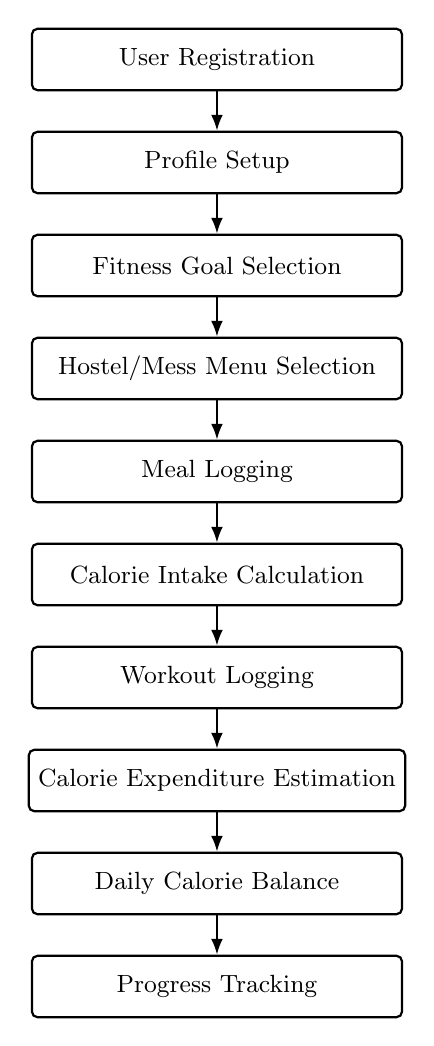
\begin{tikzpicture}[
    node distance=5mm and 9mm,
    box/.style={
        rectangle, rounded corners=2pt, draw=black, thick,
        align=center, minimum width=4.7cm, minimum height=0.78cm,
        font=\small
    },
    decision/.style={
        diamond, draw=black, thick, align=center,
        aspect=2.2, inner sep=1.5pt, font=\small
    },
    arrow/.style={-{Latex[length=2mm]}, thick}
]
\node[box] (reg) {User Registration};
\node[box, below=of reg] (profile) {Profile Setup};
\node[box, below=of profile] (goal) {Fitness Goal Selection};
\node[box, below=of goal] (menu) {Hostel/Mess Menu Selection};
\node[box, below=of menu] (meal) {Meal Logging};
\node[box, below=of meal] (intake) {Calorie Intake Calculation};
\node[box, below=of intake] (workout) {Workout Logging};
\node[box, below=of workout] (expend) {Calorie Expenditure Estimation};
\node[box, below=of expend] (balance) {Daily Calorie Balance};
\node[box, below=of balance] (progress) {Progress Tracking};

\draw[arrow] (reg) -- (profile);
\draw[arrow] (profile) -- (goal);
\draw[arrow] (goal) -- (menu);
\draw[arrow] (menu) -- (meal);
\draw[arrow] (meal) -- (intake);
\draw[arrow] (intake) -- (workout);
\draw[arrow] (workout) -- (expend);
\draw[arrow] (expend) -- (balance);
\draw[arrow] (balance) -- (progress);
\end{tikzpicture}
\end{center}

\subsection*{Step 1: User Profile}
The user creates an account and enters relevant information required for personalized calculations.

\subsection*{Step 2: Fitness Goal}
The user selects a goal such as weight loss, muscle gain, or general fitness.

\subsection*{Step 3: Mess Menu}
The application provides the available hostel mess menu instead of requiring the user to search for food items individually.

\subsection*{Step 4: Meal Logging}
The student selects the meals consumed during the day.

\subsection*{Step 5: Calorie Calculation}
The application estimates the total calories consumed based on the selected meals.

\subsection*{Step 6: Workout Logging}
The student records the workout or physical activity performed.

\subsection*{Step 7: Expenditure Calculation}
The system estimates calories burned through the recorded activity.

\subsection*{Step 8: Daily Analysis}
The system compares calorie intake and expenditure to provide a simple representation of the user's daily calorie balance.

\subsection*{Step 9: Progress Analysis}
Historical information is used to display weight changes, weekly statistics, and overall progress.

\section{Software Development Pipeline}

The development of HostelFit follows a structured software engineering pipeline that connects requirements, system modelling, implementation, verification, and deployment. The planned workflow is illustrated below.

\begin{center}
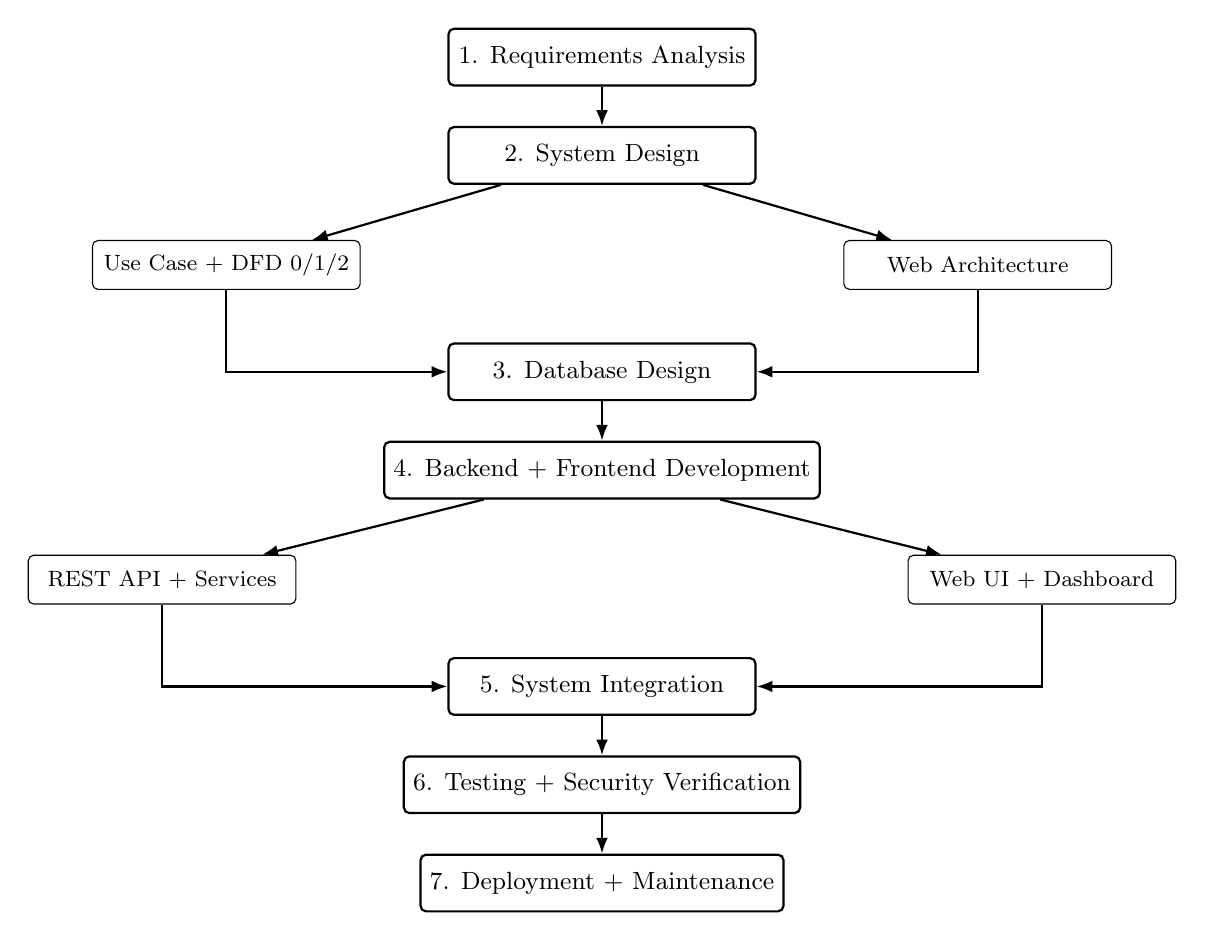
\begin{tikzpicture}[
    node distance=5mm and 7mm,
    box/.style={
        rectangle, rounded corners=2pt, draw=black, thick,
        align=center, minimum width=3.9cm, minimum height=0.72cm,
        font=\small
    },
    smallbox/.style={
        rectangle, rounded corners=2pt, draw=black,
        align=center, minimum width=3.4cm, minimum height=0.62cm,
        font=\footnotesize
    },
    arrow/.style={-{Latex[length=2mm]}, thick}
]
\node[box] (req) {1. Requirements Analysis};
\node[box, below=of req] (design) {2. System Design};
\node[smallbox, below left=7mm and 11mm of design] (uc) {Use Case + DFD 0/1/2};
\node[smallbox, below right=7mm and 11mm of design] (arch) {Web Architecture};
\node[box, below=20mm of design] (data) {3. Database Design};
\node[box, below=of data] (impl) {4. Backend + Frontend Development};
\node[smallbox, below left=7mm and 11mm of impl] (back) {REST API + Services};
\node[smallbox, below right=7mm and 11mm of impl] (front) {Web UI + Dashboard};
\node[box, below=20mm of impl] (integration) {5. System Integration};
\node[box, below=of integration] (test) {6. Testing + Security Verification};
\node[box, below=of test] (deploy) {7. Deployment + Maintenance};

\draw[arrow] (req) -- (design);
\draw[arrow] (design) -- (uc);
\draw[arrow] (design) -- (arch);
\draw[arrow] (uc) |- (data);
\draw[arrow] (arch) |- (data);
\draw[arrow] (data) -- (impl);
\draw[arrow] (impl) -- (back);
\draw[arrow] (impl) -- (front);
\draw[arrow] (back) |- (integration);
\draw[arrow] (front) |- (integration);
\draw[arrow] (integration) -- (test);
\draw[arrow] (test) -- (deploy);
\end{tikzpicture}
\end{center}

\subsection*{Pipeline Description}
\textbf{Requirements Analysis:} The project requirements are identified from the hostel-specific problem, including meal tracking, calorie estimation, workout tracking, personalized targets, and progress monitoring.

\textbf{System Design:} Requirements are translated into the Use Case Diagram and DFD Levels 0, 1, and 2, followed by definition of the web application architecture.

\textbf{Database Design:} The required entities and relationships are defined for profiles, fitness goals, hostel/mess menus, meal records, workout records, weight history, and progress information.

\textbf{Backend and Frontend Development:} The backend provides authentication, REST APIs, and application logic, while the frontend provides the web interface for students and authorized administrators.

\textbf{System Integration:} The web interface is connected to backend services and the database so that user actions produce and retrieve real application data.

\textbf{Testing and Security Verification:} Functional, integration, interface, validation, authentication, authorization, and security checks are performed before release.

\textbf{Deployment and Maintenance:} The tested system is deployed as a web application and maintained through controlled updates and fixes.

\section{Key Features}

The proposed application will include the following features:
\begin{itemize}
    \item User registration and profile management.
    \item Fitness goal selection.
    \item Hostel and mess selection.
    \item Pre-loaded mess menus.
    \item Breakfast, lunch, dinner, and snack logging.
    \item Daily calorie intake estimation.
    \item Workout and activity logging.
    \item Calorie expenditure estimation.
    \item Personalized calorie targets.
    \item Daily calorie balance dashboard.
    \item Weight tracking.
    \item Weekly progress statistics.
    \item Historical fitness data.
    \item Simple graphical representation of progress.
\end{itemize}

\section{Scope of the Project}

The initial scope of HostelFit is focused on hostel students and their specific dietary and fitness requirements.

The system will primarily address:
\begin{itemize}
    \item Hostel mess meal tracking.
    \item Calorie intake estimation.
    \item Workout tracking.
    \item Calorie expenditure estimation.
    \item Personalized fitness targets.
    \item Weight and progress tracking.
\end{itemize}

The project can later be expanded to support additional functionality such as multiple hostel databases, customized food portions, wearable-device integration, notifications, advanced analytics, and more personalized recommendations.

\section{Expected Outcome}

The expected outcome of the project is a functional mobile application that provides hostel students with a convenient way to monitor their food intake and physical activity.

The application is expected to:
\begin{itemize}
    \item Reduce the effort required to log hostel meals.
    \item Provide better visibility into daily calorie consumption.
    \item Help students understand the relationship between food intake and physical activity.
    \item Allow students to monitor their fitness progress over time.
    \item Provide a hostel-specific alternative to generic calorie-tracking applications.
\end{itemize}

The overall objective is to make fitness tracking simpler and more realistic for students living in hostels.

\section{Benefits of the Proposed System}

HostelFit provides several potential benefits:

\textbf{Convenience:} Students can log meals directly from the hostel menu rather than manually searching for food items.

\textbf{Hostel-specific functionality:} The application is designed around the constraints of hostel mess systems rather than general dietary environments.

\textbf{Integrated tracking:} Nutrition and workouts are managed in one platform.

\textbf{Improved awareness:} Students can see their approximate calorie intake and expenditure.

\textbf{Goal-oriented monitoring:} Users can monitor their progress according to their selected fitness objectives.

\textbf{Data-driven decisions:} Weekly statistics and historical records can help users understand their progress and make more informed fitness decisions.

\section{Proposed Technology}

The project is proposed as a mobile application supported by a backend database for storing user profiles, hostel menus, meal records, workout records, and progress information.

A possible implementation can use:
\begin{itemize}
    \item \textbf{Frontend:} Mobile application framework such as Flutter or React Native.
    \item \textbf{Backend:} Node.js/Express or another suitable backend framework.
    \item \textbf{Database:} Firebase, MongoDB, or a relational database.
    \item \textbf{Authentication:} Secure user authentication system.
    \item \textbf{Data Processing:} Application logic for calorie and progress calculations.
\end{itemize}

The exact technology stack may be finalized during the implementation phase according to project requirements and development constraints.



\section{Conclusion}

HostelFit proposes a practical solution to a specific problem faced by hostel students: managing nutrition and fitness despite fixed mess menus and busy schedules.

By combining hostel-specific meal tracking, calorie estimation, workout recording, personalized targets, and progress insights, the proposed application can provide students with a single platform for managing their fitness journey.

The project aims to transform fixed hostel meal schedules from an obstacle into useful, trackable information and provide students with a simpler and more actionable way to work toward their fitness goals.

\end{document}
